%!TEX root = Main.tex
\section{Theory}

\subsection{Image}
We use the $256 \times 256$ pixel grayscale cameraman image (Figure \ref{fig:image_cameraman}). The image is saved in the TelosB flash as a binary file. Each pixel is represented with one byte, which gives a grayscale resolution of 256 shades.

\begin{figure}[ht!]
\centering
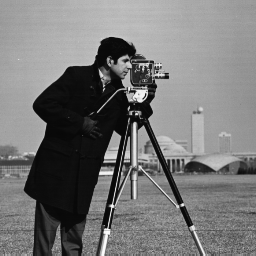
\includegraphics{cameraman}
\caption{Cameraman image used in the project.}
\label{fig:image_cameraman}
\end{figure}

\subsection{Compression}

We use three different lossy compression algorithms in this project.
They have a simple implementation and are fast to compute, but they are not very good at retaining information compared to e.g. JPEG which uses discrete cosine transform and huffman coding.

Our compression algorithms work by throwing away the least significant bit/bits from every byte in the image.
For instance the four bit compression takes two bytes, \texttt{aaaa\_\_\_\_} and \texttt{bbbb\_\_\_\_}, and compresses them to a single byte \texttt{aaaabbbb}, where \texttt{a}, \texttt{b} and \texttt{\_} is a bit. Using this method, the image has been compressed 50\%.


\subsubsection{One Bit Compression} % (fold)
\label{sub:one_bit_compression}
\FloatBarrier

The One Bit Compression gives a compression of $\dfrac{1\ bit}{8\ bit} = 12.5\%$.

The algorithm takes 8 bytes and maps them into 7 bytes where the least significant bit, of each byte, is lost. This can be seen on Figure \ref{fig:1BitCompressingAlgo}.

\begin{figure}[htbp]
	\centering
	\begin{subfigure}[t]{0.3\textwidth}\tightdisplaymath
		\centerline{
		\xymatrix@ = 2pt{
			a	& a	& a	& a	& a	& a	& a	& a	\\
			b	& b	& b	& b	& b	& b	& b	& b \\
			c	& c	& c	& c	& c	& c	& c	& c \\
			d	& d	& d	& d	& d	& d	& d	& d \\
			e	& e	& e	& e	& e	& e	& e	& e \\
			f	& f	& f	& f	& f	& f	& f	& f	\\
			g	& g	& g	& g	& g	& g	& g	& g	\\
			h	& h	& h	& h	& h	& h	& h	& h	}}
		\caption{8 uncompressed bytes.}
	\end{subfigure}
	\begin{subfigure}[t]{0.3\textwidth}\tightdisplaymath
		\centerline{
		\xymatrix@=1pt{
			a	& a	& a	& a	& a	& a	& a	& \_ \\
			b	& b	& b	& b	& b	& b	& b	& \_ \\
			c	& c	& c	& c	& c	& c	& c	& \_ \\
			d	& d	& d	& d	& d	& d	& d	& \_ \\
			e	& e	& e	& e	& e	& e	& e	& \_ \\
			f	& f	& f	& f	& f	& f	& f	& \_ \\
			g	& g	& g	& g	& g	& g	& g	& \_ \\
			h \ar[uuuuuuurrrrrrr]	& h\ar[uuuuuurrrrrr]	& h	\ar[uuuuurrrrr]& h \ar[uuuurrrr] & h \ar[uuurrr] & h \ar[uurr] & h \ar[ur] & h }}
	        \caption{Mapping from 8 to 7 bytes where LSB is lost.}
	\end{subfigure}
	\begin{subfigure}[t]{0.3\textwidth}\tightdisplaymath
		\centerline{
		\xymatrix@ = 1pt{
			a	& a	& a	& a	& a	& a	& a	& h	\\
			b	& b	& b	& b	& b	& b	& b	& h \\
			c	& c	& c	& c	& c	& c	& c	& h \\
			d	& d	& d	& d	& d	& d	& d	& h \\
			e	& e	& e	& e	& e	& e	& e	& h \\
			f	& f	& f	& f	& f	& f	& f	& h	\\
			g	& g	& g	& g	& g	& g	& g	& h	}}
		\caption{7 compressed bytes.}
	\end{subfigure}%
	\caption{One bit compressions in steps.}
	\label{fig:1BitCompressingAlgo}
\end{figure}



\subsubsection{Two bit compression} % (fold)
\label{sub:two_bit_compression}
\FloatBarrier

The Two Bit Compression losses two bits pr. byte.
This means, that a $256 \cdot 256$ pixel, 8 bit picture (65536 bytes) will be reduced $\dfrac{3}{4}$ of information (49152 bytes).
With this compression there will be 64 different (versus the original 256) colors to represent the picture.

Figure \ref{fig:2BitUncompressed} shows the 8 uncompressed bits. 
Because it is a two bit compression the last two bit are cut away from each byte, as seen on Figure \ref{fig:2bitCom}.
The last byte, \texttt{dddd dd00}, should be transfered to the end of each other byte which gives the result of Figure \ref{fig:2BitCompressed}.


\begin{figure}[htbp]
	\centering
	\begin{subfigure}[t]{0.3\textwidth}\tightdisplaymath
		\centerline{
		\xymatrix@ = 2pt{
			a	& a	& a	& a	& a	& a	& a	& a	\\
			b	& b	& b	& b	& b	& b	& b	& b \\
			c	& c	& c	& c	& c	& c	& c	& c \\
			d	& d	& d	& d	& d	& d	& d	& d }}
		
		\caption{4 uncompressed bytes.}
		\label{fig:2BitUncompressed}
	\end{subfigure}
	\begin{subfigure}[t]{0.3\textwidth}\tightdisplaymath
		\centerline{
		\xymatrix@=1pt{
			a	& a	& a	& a	& a	& a	& 0	& 0	\\
			b	& b	& b	& b	& b	& b	& 0	& 0 \\
			c	& c	& c	& c	& c	& c	& 0	& 0 \\
			d \ar[uuurrrrrr]	& d\ar[uuurrrrrr]	& d\ar[uurrrr]	& d\ar[uurrrr]	& d\ar[urr]	& d\ar[urr]	& 0	& 0 }}
		
		\caption{Replace last two bits with the 4th byte's bits.}
		\label{fig:2bitCom}
	\end{subfigure}
	\begin{subfigure}[t]{0.3\textwidth}\tightdisplaymath
		\centerline{
		\xymatrix@ = 1pt{
			a	& a	& a	& a	& a	& a	& d	& d	\\
			b	& b	& b	& b	& b	& b	& d	& d \\
			c	& c	& c	& c	& c	& c	& d	& d }}
		\caption{3 compressed bytes.}
		\label{fig:2BitCompressed}
	\end{subfigure}%
	\caption{Two bit compressions in steps.}
\end{figure}




\subsubsection{Four bit compression} % (fold)
\label{sub:four_bit_compression}
\FloatBarrier

The Four Bit Compression losses four bits pr. byte.
This means, that a $256 \cdot 256$ pixel, 8 bit picture (65536 bytes) will be reduced $\dfrac{1}{2}$ of information (32768 bytes).
With this compression there will be 32 different (versus the original 256) colors to represent the picture.

Figure \ref{fig:4BitUncompressed} shows the 8 uncompressed bits. 
Because it is a two bit compression the last two bit are cut away from each byte, as seen on Figure \ref{fig:4bitCom}.
The last byte, \texttt{bbbb 0000}, should be transfered to the end of each other byte which gives the result of Figure \ref{fig:4BitCompressed}.


\begin{figure}[htbp]
	\centering
	\begin{subfigure}[t]{0.3\textwidth}\tightdisplaymath
		\centerline{
		\xymatrix@ = 2pt{
			a	& a	& a	& a	& a	& a	& a	& a	\\
			b	& b	& b	& b	& b	& b	& b	& b }}
		
		\caption{2 uncompressed bytes.}
		\label{fig:4BitUncompressed}
	\end{subfigure}
	\begin{subfigure}[t]{0.3\textwidth}\tightdisplaymath
		\centerline{
		\xymatrix@=1pt{
			a	& a	& a	& a	& 0	& 0	& 0	& 0	\\
			b \ar[urrrr] & b\ar[urrrr] & b\ar[urrrr] & b \ar[urrrr] & 0	& 0	& 0	& 0 }}
		
		\caption{Replace last four bits with the 2nd byte's bits.}
		\label{fig:4bitCom}
	\end{subfigure}
	\begin{subfigure}[t]{0.3\textwidth}\tightdisplaymath
		\centerline{
		\xymatrix@ = 1pt{
			a	& a	& a	& a	& b	& b	& b	& b	}}
		\caption{1 compressed byte.}
		\label{fig:4BitCompressed}
	\end{subfigure}%
	\caption{Four bit compressions in steps.}
\end{figure}



